\section{Problem Statement}

% \subsection{Motivation}

\begin{frame}
  \frametitle{Motivation}
  \begin{itemize}
    \item Protecting information in contested and congested wireless communication environments requires transmissions that are difficult to intercept or even detect (LPI/LPD). 
     \item A key measure to achieve robust protection against detection is to rely on signals with power spectral densities that are well below the noise floor. 
     % \item To recover the signals at low SNR, joint detection and carrier synchronization algorithms play a vital role in protected communication system. 
     \item At low SNR, the time and carrier synchronization are coupled problems: coherent methods for detecting the signal require accurate carrier estimations while data-aided carrier estimation requires the location of the training sequence is available.
     \item In practice, the position of the embedded training sequence (preamble) should be searched sequentially.
 
 \end{itemize}
\end{frame}

% \subsection{Previous Work}

\begin{frame}
    \frametitle{Previous Work}
    \begin{itemize}
        \item Some classical works on carrier synchronization were discussed by assuming time synchronization has been accomplished~\cite{Morelli_Mengali_98}. However, this is not reliable especially at low SNR.
        \item The time and carrier synchronization were performed jointly with good accuracy at low SNR in~\cite{purushothaman_16,kim_17}. However, they were doing frame synchronization and the relative
        computation is high.
        \item Computational complexity is another major concern with the practical realization of a synchronization system discussed in~\cite{murin_16,wang_21}.
    
    \end{itemize}
  \end{frame}



\begin{frame}
    \frametitle{Our Research}
    \begin{itemize}
        \item Our research provides a comprehensive treatment of the signal acquisition problem of protected communications, which basically includes
        \begin{itemize}
            \item a family of joint detection and estimation algorithm that emphasize computational complexity while maintaining near-optimal accuracy at very low SNR, and
            \item the implementation of the proposed algorithms on a standard SDR platform.
        \end{itemize} 
    \end{itemize}

    \begin{figure}
        \centering
        \begin{minipage}{.5\textwidth}
          \centering
          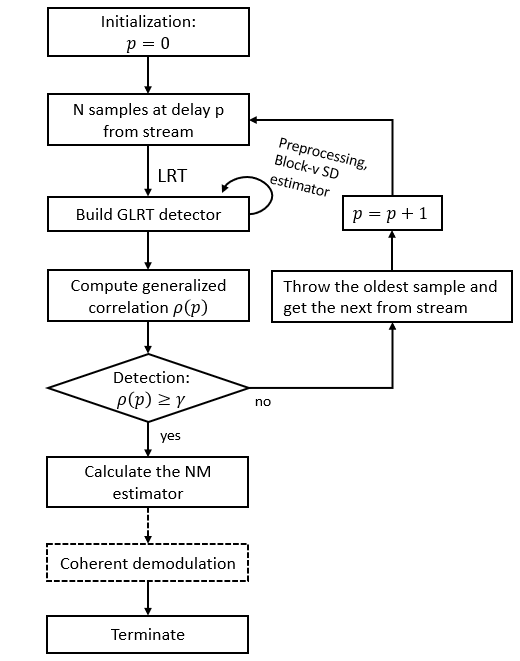
\includegraphics[width=.5\linewidth]{architecture_of_paper.png}
        \end{minipage}%
        \begin{minipage}{.5\textwidth}
          \centering
          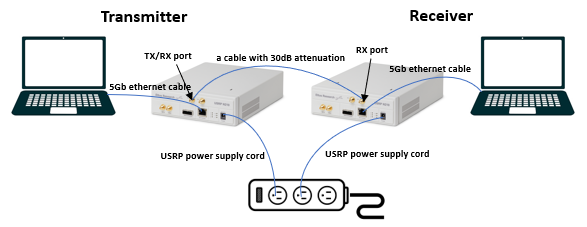
\includegraphics[width=.8\linewidth]{SDR_signal_transmission_path.png}
        \end{minipage}
    \end{figure}

\end{frame}

